\section{Gradient-Based Optimization}
\label{sec:theory:optimization}

In machine learning one often wish to minimize a loss function that is not easily optimizable. Such a loss function can be misclassification rate or the BLEU score which is commonly used in translation. Because these loss functions are hard to optimize directly a similar loss function like cross-entropy is often used. Loss functions like cross-entropy are easily differentiable which makes it feasible to optimize them.

Modern neural networks typically have a large number of weights, the ByteNet model which will later be used for natural language translation has approximately 27 million parameters. Classical optimization methods typically use the second-order derivative of the loss function such as the Newton method or use an approximation like the Quasi-Newton method. However, because the second-order derivative matrix (the Hessian), or even just approximations of it, scales quadratically with the number of weights, it is not feasible to use the second-order derivative for optimizing neural networks.

Because of the many weights in neural networks, optimization is typically done using only the gradient, this is known as \textit{gradient-based optimization}.

The fundamental principal in \textit{gradient-based optimization} is to initialize the parameters, typically this will be done randomly. The parameters are then optimized by iteratively going in the opposite direction of the gradient of the loss function with respect to the parameters.

\begin{equation}
\mathbf{w}_t = \mathbf{w}_{t-1} - {\boldsymbol\Delta}_t, \quad {\boldsymbol\Delta}_t = \alpha \frac{\partial \mathcal{L}(\mathbf{w}_{t-1})}{\partial \mathbf{w}_{t-1}}
\label{eq:theory:optimization:batch-optimization}
\end{equation}

Here $\mathbf{w}_t$ is a vector containing all the model weights at iteration $t$, ${\boldsymbol\Delta}_t$ is the step taken, and $\alpha$ is called the \textit{step size} or \textit{learning rate}. The learning rate $\alpha$ should be small enough such that the step doesn't jump over the minima, but also big enough such that the model gets optimized within reasonable time.

It is important to understand that even if the global minima is found, $\mathcal{L}(\mathbf{w}_{t-1})$ is not the true loss function, it is just the loss function given a training dataset. Hopefully, the training dataset is an accurate representation of reality, but this is not possible to guarantee. To validate the model, a test dataset that is not a part of the training dataset is used.

It is often the case that the minima when using the training dataset is not the minima when using the test dataset. The typical behavior, is that the training loss will continue to decrease because that is what is being optimized, while the test loss will only decrease initially and then increase later. This behavior is called overfitting, there are numerous ways to prevent this, some of which will be discussed and used throughout this thesis.

\begin{figure}[h]
    \centering
    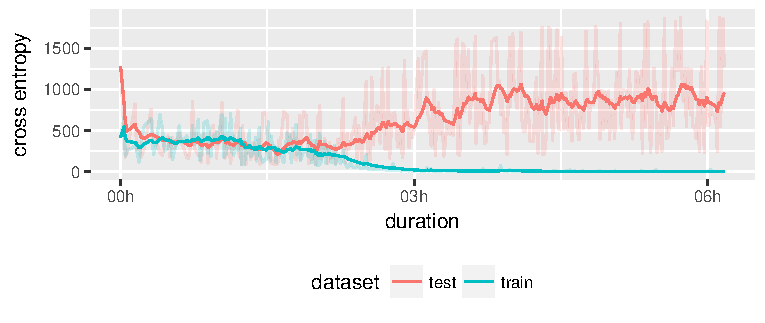
\includegraphics[scale=1]{theory/overfitting.pdf}
    \caption{Shows the ByteNet model overfitting. The semi-transparent line is the loss, and the non-transparent line is an exponential moving average of the loss.}
\end{figure}

\subsection{Stochastic Optimization}

While the approach in \eqref{eq:theory:optimization:batch-optimization} can work, it is often not feasible to calculate $\frac{\partial \mathcal{L}(\mathbf{w}_{t-1})}{\partial \mathbf{w}_{t-1}}$ on the entire dataset. For a model with a huge number of parameters, it is typically necessary to also have a very large dataset. To solve this problem $\frac{\partial \mathcal{L}(\mathbf{w}_{t-1})}{\partial \mathbf{w}_{t-1}}$ is estimated using a random sample of observations in each iteration. This approach is called \textit{minibatch stochastic gradient descent} or just \textit{minibatch learning} \cite{deep-learning}.

Beyond making the computation feasible this also has some advantages:

\begin{itemize}
\item Consider two datasets one with 256 observations and another with 16 observations. It will take 16 times more time to calculate the gradient using 256 observations than 16 observations. However, because of the square-root law, it only decreases the standard error by a factor of 4. It is thus likely to be more economical to perform 16 as many iterations, than being 4 times more accurate.

\item It is typically easy to parallelize over observations. For a multi-parallel hardware like a GPU it is typically possible to parallelize over many observations without extra cost. For large networks, it is common to estimate the gradient approximately 16 observations.

\item Sampling observations from a dataset adds noise to the gradients. This noise can have a regularizing effect on the training, causing less overfitting \cite{deep-learning}.
\end{itemize}

The stochastic part of \textit{minibatch stochastic gradient descent} comes from the fact that $\frac{\partial \mathcal{L}(\mathbf{w}_{t-1})}{\partial \mathbf{w}_{t-1}}$ is no longer the same in each iteration. Because the gradient is estimated from a new random sample of observations from the dataset, $\frac{\partial \mathcal{L}(\mathbf{w}_{t-1})}{\partial \mathbf{w}_{t-1}}$ is essentially samples from a random distribution. The changes the minimization problem from minimizing $\mathcal{L}$ to minimizing the expectation $\mathbb{E}[\mathcal{L}]$. Minibatch learning does not directly tackle this change of problem type, it just causes it. To correctly optimize a stochastic loss function more advanced optimization methods are needed.

\subsection{Adam Optimization}

Adam optimization is a gradient-based optimization method for optimizing a stochastic loss function, it has been shown to work well both theoretically and empirically. It even works on a stochastic loss function with changing distribution. Changing distribution is something that is quite common when changing the parameters of the model, thus this is an important property \cite{adam-optimization}.

The central idea of Adam optimization is to scale the step-size by a signal-to-noise estimate. Such that when the signal is strong a large step is taken and when it is weak a small step is taken. This is accomplished by having a running estimate of the first and second moment.
\begin{equation}
\begin{aligned}
\mathbf{g}_t &= \frac{\partial \mathcal{L}(\mathbf{w}_{t-1})}{\partial \mathbf{w}_{t-1}} \\
\mathbf{m}_t &= \beta_1 \mathbf{m}_{t-1} + (1 - \beta_1) \mathbf{g}_t \\
\mathbf{v}_t &= \beta_2 \mathbf{v}_{t-1} + (1 - \beta_2) \mathbf{g}_t^2
\end{aligned}
\end{equation}

The ``signal-to-noise'' ratio as the original paper \cite{adam-optimization} calls it, is then calculated as $\frac{\mathbf{m}_t}{\sqrt{\mathbf{v}_t}}$. Calling  $\frac{\mathbf{m}_t}{\sqrt{\mathbf{v}_t}}$ a ``signal-to-noise'' ratio is a slight abuse of terminology, because $\mathbf{v}_t$ is not exactly a variance estimate, but the effect is similar.

A problem that remains is how to initialize $\mathbf{m}_{0}$ and $\mathbf{v}_{0}$. The solution is to initialize them as zero. Since zero is what the gradient will converge to, this is not unreasonable, however to improve the estimates they are rescaled to be unbiased.

Consider the second-order moment at iteration $t$, this can be directly expressed as:
\begin{equation}
\mathbf{v}_t = (1 - \beta_2)\sum_{i=1}^t \beta_2^{t-i} \mathbf{g}_{i}^2
\end{equation}

To make the $\mathbf{v}_t$ estimate unbiased the relation between $\mathbb{E}[\mathbf{v}_t]$ and $\mathbb{E}[\mathbf{g}_t^2]$ should be calculated. Assuming the distribution of $\mathbb{E}[\mathbf{g}_t^2]$ is stationary the relation is: 
\begin{equation}
\begin{aligned}
\mathbb{E}[\mathbf{v}_t] &= \mathbb{E}\left[(1 - \beta_2)\sum_{i=1}^t \beta_2^{t-i} \mathbf{g}_{i}^2\right]
= (1 - \beta_2)\sum_{i=1}^t \beta_2^{t-i} \mathbb{E}\left[\mathbf{g}_{i}^2\right] \\
&= \mathbb{E}\left[\mathbf{g}_{i}^2\right] (1 - \beta_2)\sum_{i=1}^t \beta_2^{t-i}
= \mathbb{E}\left[\mathbf{g}_{i}^2\right] (1 - \beta_2^t)
\end{aligned}
\end{equation}

Thus to unbias the $\mathbf{v}_t$ estimate it is scaled by $\frac{1}{1 - \beta_2^t}$, similarly $\mathbf{m}_t$ re scaled by $\frac{1}{1 - \beta_1^t}$:
\begin{equation}
\begin{aligned}
\hat{\mathbf{m}}_t = \frac{1}{1 - \beta_1^t} \mathbf{m}_t, \quad \hat{\mathbf{v}}_t = \frac{1}{1 - \beta_2^t} \mathbf{v}_t
\end{aligned}
\label{eq:theory:optimization:adam-unbias}
\end{equation}

The parameter update is then done as follow:
\begin{equation}
\begin{aligned}
{\boldsymbol\Delta}_t &= \alpha \frac{\hat{\mathbf{m}}_t}{\sqrt{\hat{\mathbf{v}}_t} + \epsilon} \mathbf{g}_t \\
\mathbf{w}_t &= \mathbf{w}_{t-1} - {\boldsymbol\Delta}_t
\end{aligned}
\label{eq:theory:optimization:adam-update}
\end{equation}

Computationally this can be done slightly more efficient by combining \eqref{eq:theory:optimization:adam-unbias} with \eqref{eq:theory:optimization:adam-update}:
\begin{equation}
{\boldsymbol\Delta}_t = \alpha \frac{\sqrt{1 - \beta_2^t}}{1 - \beta_1^t} \frac{\mathbf{m}_t}{\sqrt{\mathbf{v}_t} + \epsilon} \mathbf{g}_t
\end{equation}


\begin{algorithm}[H]
  \caption{Adam Optimization, default parameters are $\alpha=0.001, \beta_1=0.9, \beta_2=0.999, \epsilon=10^{-8}$}
  \begin{algorithmic}[1]
    \Function{Adam}{$\mathcal{L}(\mathbf{w}), \mathbf{w}_0, \alpha, \beta_1, \beta_2, \epsilon$}
      \Let{$\mathbf{m}_0$}{\Call{ZeroLike}{$\mathbf{w}$}}
      \Let{$\mathbf{v}_0$}{\Call{ZeroLike}{$\mathbf{w}$}}
      \Let{$t$}{$0$}
      \Repeat
        \Let{$t$}{$t + 1$}
        \Let{$\mathbf{g}_t$}{$\frac{\partial \mathcal{L}(\mathbf{w}_{t-1})}{\partial \mathbf{w}_{t-1}}$}
        \Let{$\mathbf{m}_t$}{$\beta_1 \mathbf{m}_{t-1} + (1 - \beta_1) \mathbf{g}_t$}
        \Let{$\mathbf{v}_t$}{$\beta_2 \mathbf{v}_{t-1} + (1 - \beta_2) \mathbf{g}_t^2$}
        \Let{${\boldsymbol\Delta}_t$}{$\alpha \frac{\sqrt{1 - \beta_2^t}}{1 - \beta_1^t} \frac{\mathbf{m}_t}{\sqrt{\mathbf{v}_t} + \epsilon} \mathbf{g}_t$}
        \Let{$\mathbf{w}_t$}{$\mathbf{w}_{t-1} - {\boldsymbol\Delta}_t$}
      \Until{converged}
      \State \Return{$\mathbf{w}_t$}
    \EndFunction
  \end{algorithmic}
\end{algorithm}

\subsection{He-Uniform Initialization}

An open question that has not been answered is how to initialize the weights $\mathbf{w}_0$. This turns out to very much depend on the architecture, the ByteNet model that will be used later is a convolutional model with ReLU activation. For this kind of architecture, \textit{He initialization} has been shown to perform well \cite{he-initialization}. 

Good initialization is required to prevent either exploding or vanishing gradients. Consider both the forward and backward pass for a feed forward neural network.
\begin{equation}
\begin{aligned}
z_{h_\ell} &= \sum_{h_{\ell-1} = 1}^{H_{\ell-1}} w_{h_{\ell-1}, h_{\ell}} a_{h_{\ell-1}} + b_{h_{\ell}}, a_{h_\ell} = \theta(z_{h_\ell}) \\
\delta_{h_\ell} &= \theta'(z_\ell) \sum_{h_{\ell+1}}^{H_{\ell+1}} \delta_{h_{\ell+1}} w_{h_\ell, h_{\ell+1}}
\end{aligned}
\end{equation}

In both cases, the output of layer $\ell$ ($z_{h_\ell}$ and $\delta_{h_\ell}$) depends on the output of the previous or next layer ($z_{h_{\ell-1}}$ and $\delta_{h_{\ell-1}}$). If both $z_{h_\ell}$ and $\delta_{h_\ell}$ does not maintain the same scale throughout all the layers, the values will diverge either to very small (vanishing) or very big values (exploding).

Since the values of input are unknown and the weights are to be initialized randomly, one needs to analyze $z_{h_\ell}$ and $\delta_{h_\ell}$ as stochastic variables. Keeping the expectation at a constant scale for all layers is not a huge problem, the biases $b_{h_\ell}$ are initialized to zero (not random), and the weights $w_{h_{\ell-1}, h_\ell}$ should have zero mean and be independently sampled. Likewise, it is for the analysis assumed that the inputs $a_{h_0}$ also are independent, but they do not necessarily have zero mean.
\begin{equation}
\begin{aligned}
\mathbb{E}[z_{h_\ell}]
&= H_{\ell-1} \mathbb{E}[w_{h_{\ell-1}, h_{\ell}} a_{h_{\ell-1}} + b_{h_\ell}] = H_{\ell-1} \left(\mathbb{E}[w_{h_{\ell-1}, h_{\ell}}] \mathbb{E}[a_{h_{\ell-1}}] + \mathbb{E}[b_{h_\ell}]\right) \\
&= H_{\ell-1}\left(\cdot 0 \cdot \mathbb{E}[a_{h_{\ell-1}}] + 0\right) = 0 \\
\mathbb{E}[\delta_{h_\ell}] &= \mathbb{E}[\theta'(z_\ell)] H_{\ell + 1} \mathbb{E}[\delta_{h_{\ell+1}}] \mathbb{E}[w_{h_\ell, h_{\ell+1}}] \\
&= \mathbb{E}[\theta'(z_\ell)] H_{\ell + 1} \mathbb{E}[\delta_{h_{\ell+1}}] \cdot 0 = 0
\end{aligned}
\end{equation}

It turns out that to get a good initialization it is also necessary to keep a constant variance for all layers \cite{glorot-initialization, he-initialization}. To do this correctly it is necessary to know the activation function. An often used approach is the Glorot initialization \cite{glorot-initialization}, however this assumes the activation function is linear around $z_{h_\ell} = 0$ which is not the case for ReLU ($max(0, z_{h_{\ell}})$). He initialization has later been derived specifically for the ReLU activation function \cite{he-initialization}.

The variance for the forward pass is:
\begin{equation}
\mathrm{Var}[z_{h_\ell}] = H_{\ell-1} \mathrm{Var}[w_{h_{\ell-1}, h_{\ell}} a_{h_{\ell-1}}]
\end{equation}

Because $w_{h_{\ell-1}, h_{\ell}}$ has zero mean this can be rewritten as:
\begin{equation}
\begin{aligned}
\mathrm{Var}[z_{h_\ell}]
&= H_{\ell-1} \left( \mathbb{E}[w_{h_{\ell-1}, h_{\ell}}^2 a_{h_{\ell-1}}^2] - \mathbb{E}[w_{h_{\ell-1}, h_{\ell}} a_{h_{\ell-1}}]^2 \right) \\
&= H_{\ell-1} \mathbb{E}[w_{h_{\ell-1}, h_{\ell}}^2] \mathbb{E}[a_{h_{\ell-1}}^2] \\
&= H_{\ell-1} \left(\mathrm{Var}[w_{h_{\ell-1}, h_{\ell}}] + \mathbb{E}[w_{h_{\ell-1}, h_{\ell}}]^2\right) \mathbb{E}[a_{h_{\ell-1}}^2] \\
&= H_{\ell-1} \mathrm{Var}[w_{h_{\ell-1}, h_{\ell}}] \mathbb{E}[a_{h_{\ell-1}}^2]
\end{aligned}
\end{equation}

If additionally the $w_{h_{\ell-1}, h_{\ell}}$ distribution is chosen to be symmetric around zero, then $z_{h_\ell}$ will also be symmetric around zero, call this distribution $p(z_{h_\ell}) = p(-z_{h_\ell})$, then it can be derived that $\mathbb{E}[a_{h_\ell}^2] = \frac{1}{2} \mathrm{Var}[z_{h_\ell}]$.
\begin{equation*}
\begin{aligned}
\mathbb{E}[a_{h_\ell}^2] &= \int_{-\infty}^\infty \max(0,z_{h_\ell})^2 p(z_{h_\ell}) \mathrm{d}z_{h_\ell}
&&= \int_{-\infty}^0 0^2 p(z_{h_\ell}) \mathrm{d}z_{h_\ell}
 + \int_{0}^\infty z_{h_\ell}^2 p(z_{h_\ell}) \mathrm{d}z_{h_\ell} \\
&= \int_{0}^\infty z_{h_\ell}^2 p(z_{h_\ell}) \mathrm{d}z_{h_\ell}
&&= \frac{1}{2} \int_{-\infty}^\infty z_{h_\ell}^2 p(z_{h_\ell}) \mathrm{d}z_{h_\ell} \\
&= \frac{1}{2} \mathbb{E}[z_{h_\ell}^2] = \frac{1}{2} \left(\mathbb{E}[z_{h_\ell}^2] - \mathbb{E}[z_{h_\ell}]^2\right) &&= \frac{1}{2} \mathrm{Var}[z_{h_\ell}]
\end{aligned}
\end{equation*}

Applying $\mathbb{E}[a_{h_{\ell-1}}^2] = \frac{1}{2} \mathrm{Var}[z_{h_{\ell-1}}]$ to $\mathrm{Var}[z_{h_\ell}]$ yields:
\begin{equation}
\begin{aligned}
\mathrm{Var}[z_{h_\ell}] &= H_{\ell-1} \mathrm{Var}[w_{h_{\ell-1}, h_{\ell}}] \frac{1}{2} \mathrm{Var}[z_{h_{\ell-1}}] \\
&= \mathrm{Var}[z_{h_1}] \prod_{\ell=2}^L H_{\ell-1} \frac{1}{2} \mathrm{Var}[w_{h_{\ell-1}, h_{\ell}}]
\end{aligned}
\label{eq:theory:optimize:he-all-var}
\end{equation}

From \eqref{eq:theory:optimize:he-all-var} it seen that to satisfy a constant variance ($\mathrm{Var}[z_{h_\ell}] = \mathrm{Var}[z_{h_1}]$), it is sufficient to have ${H_{\ell-1} \frac{1}{2} \mathrm{Var}[w_{h_{\ell-1}, h_{\ell}}] = 1}$.
\begin{equation}
\mathrm{Var}[w_{h_{\ell-1}, h_{\ell}}] = \frac{2}{H_{\ell-1}}
\end{equation}

The same sufficient condition is found by analyzing the backward pass \cite{he-initialization}.

Thus long as the sampling distribution has zero mean, is symmetric, is sampled independently, and has variance $\frac{2}{H_{\ell-1}}$, there shouldn't be any convergence issues. Two normal choices are the normal distribution and the uniform distribution. An issue with using the normal distribution is that there is a small risk that extreme values will be sampled, which can cause issues. A truncated normal distribution could be used to solve this issue, but a much simpler solution is to just use a uniform distribution.

A uniform distribution from $-r$ to $r$ has variance:
\begin{equation}
\mathrm{Var}[w_{h_{\ell-1}, h_{\ell}}] = \frac{1}{12} (r - (-r))^2 = \frac{1}{3} r^2
\end{equation}
Thus the uniform distribution parameter should be:
\begin{equation}
r = \sqrt{\frac{6}{H_{\ell-1}}}
\end{equation}

Note, $H_{\ell-1}$ is only valid in some cases. In other cases such the number of weights used in the activation sum may be greater or less than $H_{\ell-1}$. In general, $\mathrm{fan}_{\ell, in}$ is used instead of $H_{\ell-1}$.
